
\begin{saveblock}{otherMathNotations}
	\begin{highlightblock}[gobble=8,linewidth=0.5\textwidth,
		framexleftmargin=0.25em,xleftmargin=0.25em]
		AA \(\sqrt{2}\)
		BB \[\sqrt{3}\]
		CC $$ \sqrt{4} $$
	\end{highlightblock}
\end{saveblock}

\addtorecentlist{\textbackslash [ \textellipsis\textbackslash]}

\begin{frame}{\lang,Also in use,Ook in gebruik,}
	\begin{columns}
		\begin{column}{0.5\textwidth}
			\useblock{otherMathNotations}
		\end{column}
		\begin{column}{0.5\textwidth}
			\fbox{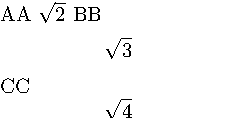
\includegraphics[width=\linewidth-2\fboxrule-2\fboxsep,height=0.9\textheight,keepaspectratio]{assets/mathOtherNotations.pdf}}
		\end{column}
	\end{columns}

	% \useblock{otherMathNotations}

	% 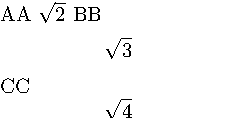
\includegraphics[width=\linewidth,height=0.4\textheight,keepaspectratio]{assets/mathOtherNotations.pdf}
\end{frame}
